\newpage
\section{3次元の気泡上昇流れ問題}

二層流の別のベンチマーク問題として3次元の気泡上昇流れ問題を解析し、参考文献の結果と比較した。

\subsection{解析条件}

Table \ref{table:3d-bubble-material-property}に二つの流体の物性値、Table \ref{table:3d-bubble-parameter}に解析パラメータを示す。
モートン数$Mo = \frac{(\rho_L-\rho_G)g \mu_L^4 }{\rho_L^2 \sigma^3}$
エトベス数$Eo = \frac{(\rho_L-\rho_G) g d^2}{\sigma}$


この式もある$Eo = \frac{4\rho_1 g (r_0)^2}{\sigma}$
ここで$d$は代表長さで気泡直径。

\renewcommand{\arraystretch}{1}
\begin{table}[H]
	\centering
	\caption{解析パラメータ}
	\begin{tabular}{cccccccccc}
		\hline
		Test case & $\rho_1$ & $\rho_2$ & $\mu_1$ & $\mu_2$ & $\mathrm{g}$ & $\sigma$ & $Eo$ & $Mo$ \\
		\hline 
		Case$1$ & $1000$ & $100$ & $10$ & $1$   & $0.98$ & $24.5$ & $9.0$ & $0.36$\\
		Case$2$ & $1000$ & $1$   & $10$ & $0.1$ & $0.98$ & $1.96$ & $125$ & $5.0$\\ 
		\hline         
	\end{tabular}
	\label{table:3d-bubble-material-property}
\end{table}
\renewcommand{\arraystretch}{1.0}

Case1は表面張力が強いため、数値安定性のために$\tau$を小さくする必要がある。\cite{Yamaguchi2018}


\renewcommand{\arraystretch}{1}
\begin{table}[H]
	\centering
	\caption{解析パラメータ}
	\begin{tabular}{ccc}
		\hline
		Test case & メッシュ幅$dx$ & 界面幅$D$\\
		\hline 
		Case$1$ & $0.05$ & $0.05$\\
		\hline         
	\end{tabular}
	\label{table:3d-bubble-parameter}
\end{table}
\renewcommand{\arraystretch}{1.0}

Figure \ref{fig:3d-bubble-setting}に文献\cite{Safi2017}から引用した解析領域の図を示す。

\begin{figure}[H]
	\centering
	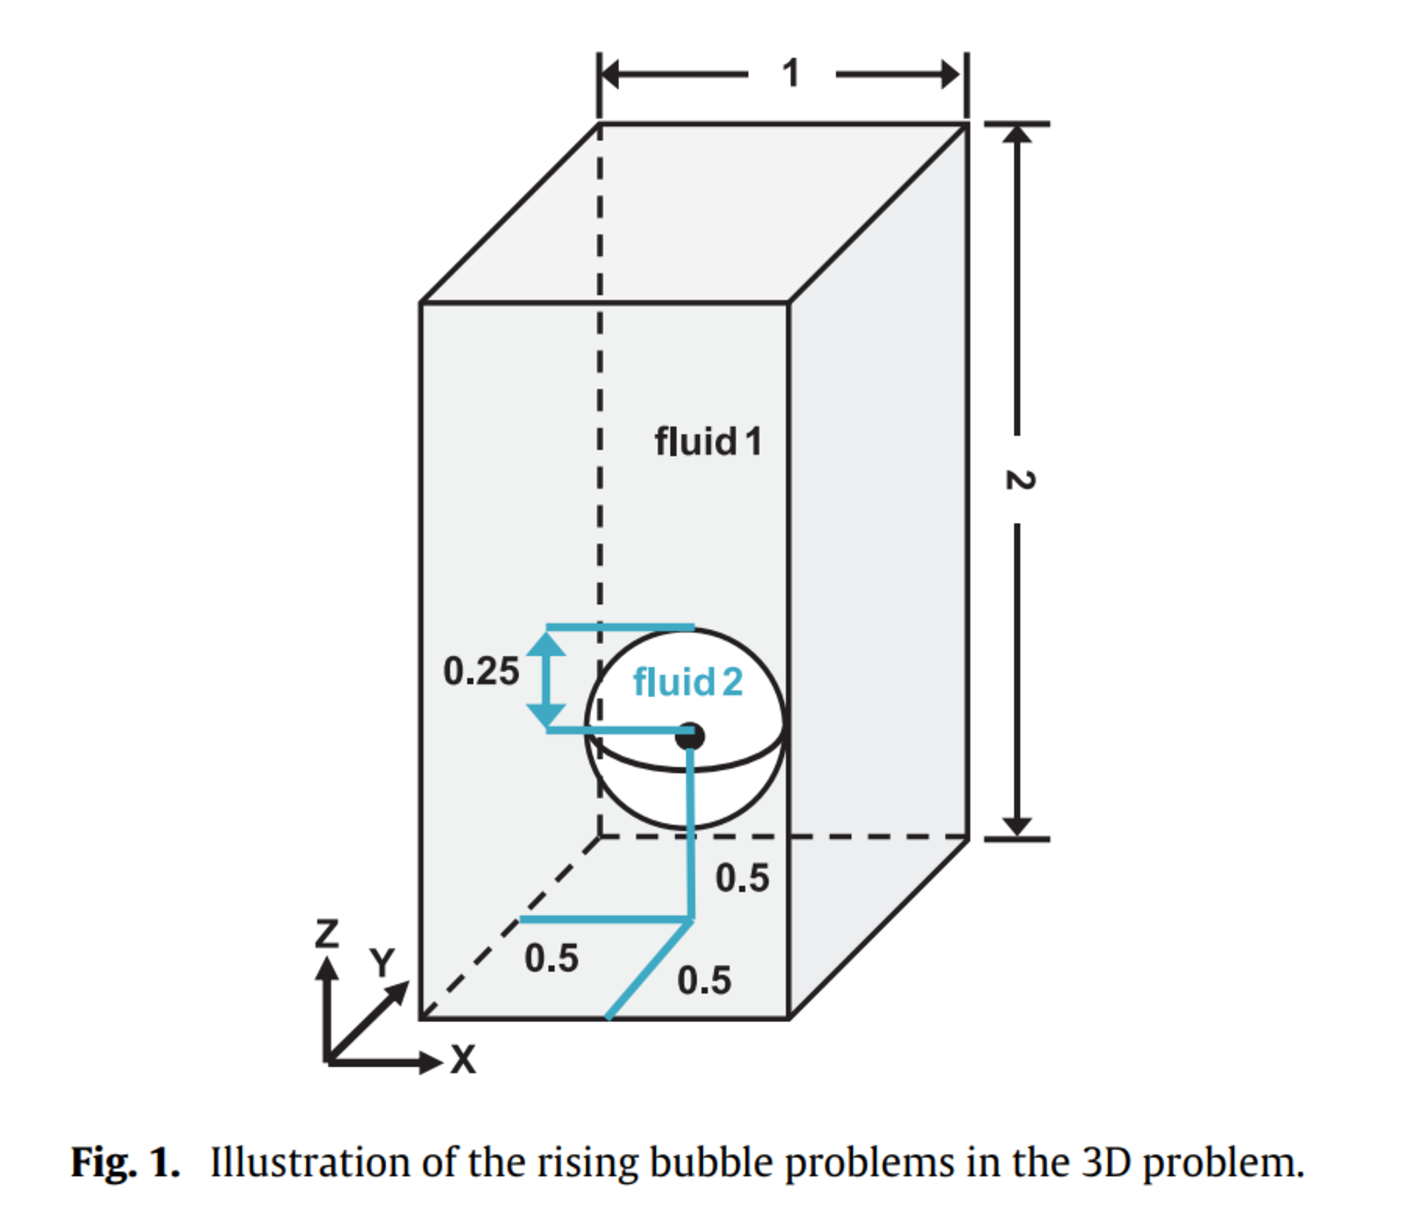
\includegraphics[width=10truecm]{pics/3d-bubble/setting.pdf}
	\caption{解析条件\cite{Safi2017}}
	\label{fig:3d-bubble-setting}
\end{figure}

Figure \ref{fig:3d-bubble-mesh}に解析用のメッシュを示す。メッシュは四面体$1$次要素を使用した。境界条件はダムブレイク問題と同様に上面を流出境界条件として圧力のディリクレ境界条件$p=0$、それ以外の面を滑りなし壁境界とした。

\begin{figure}[H]
	\centering
	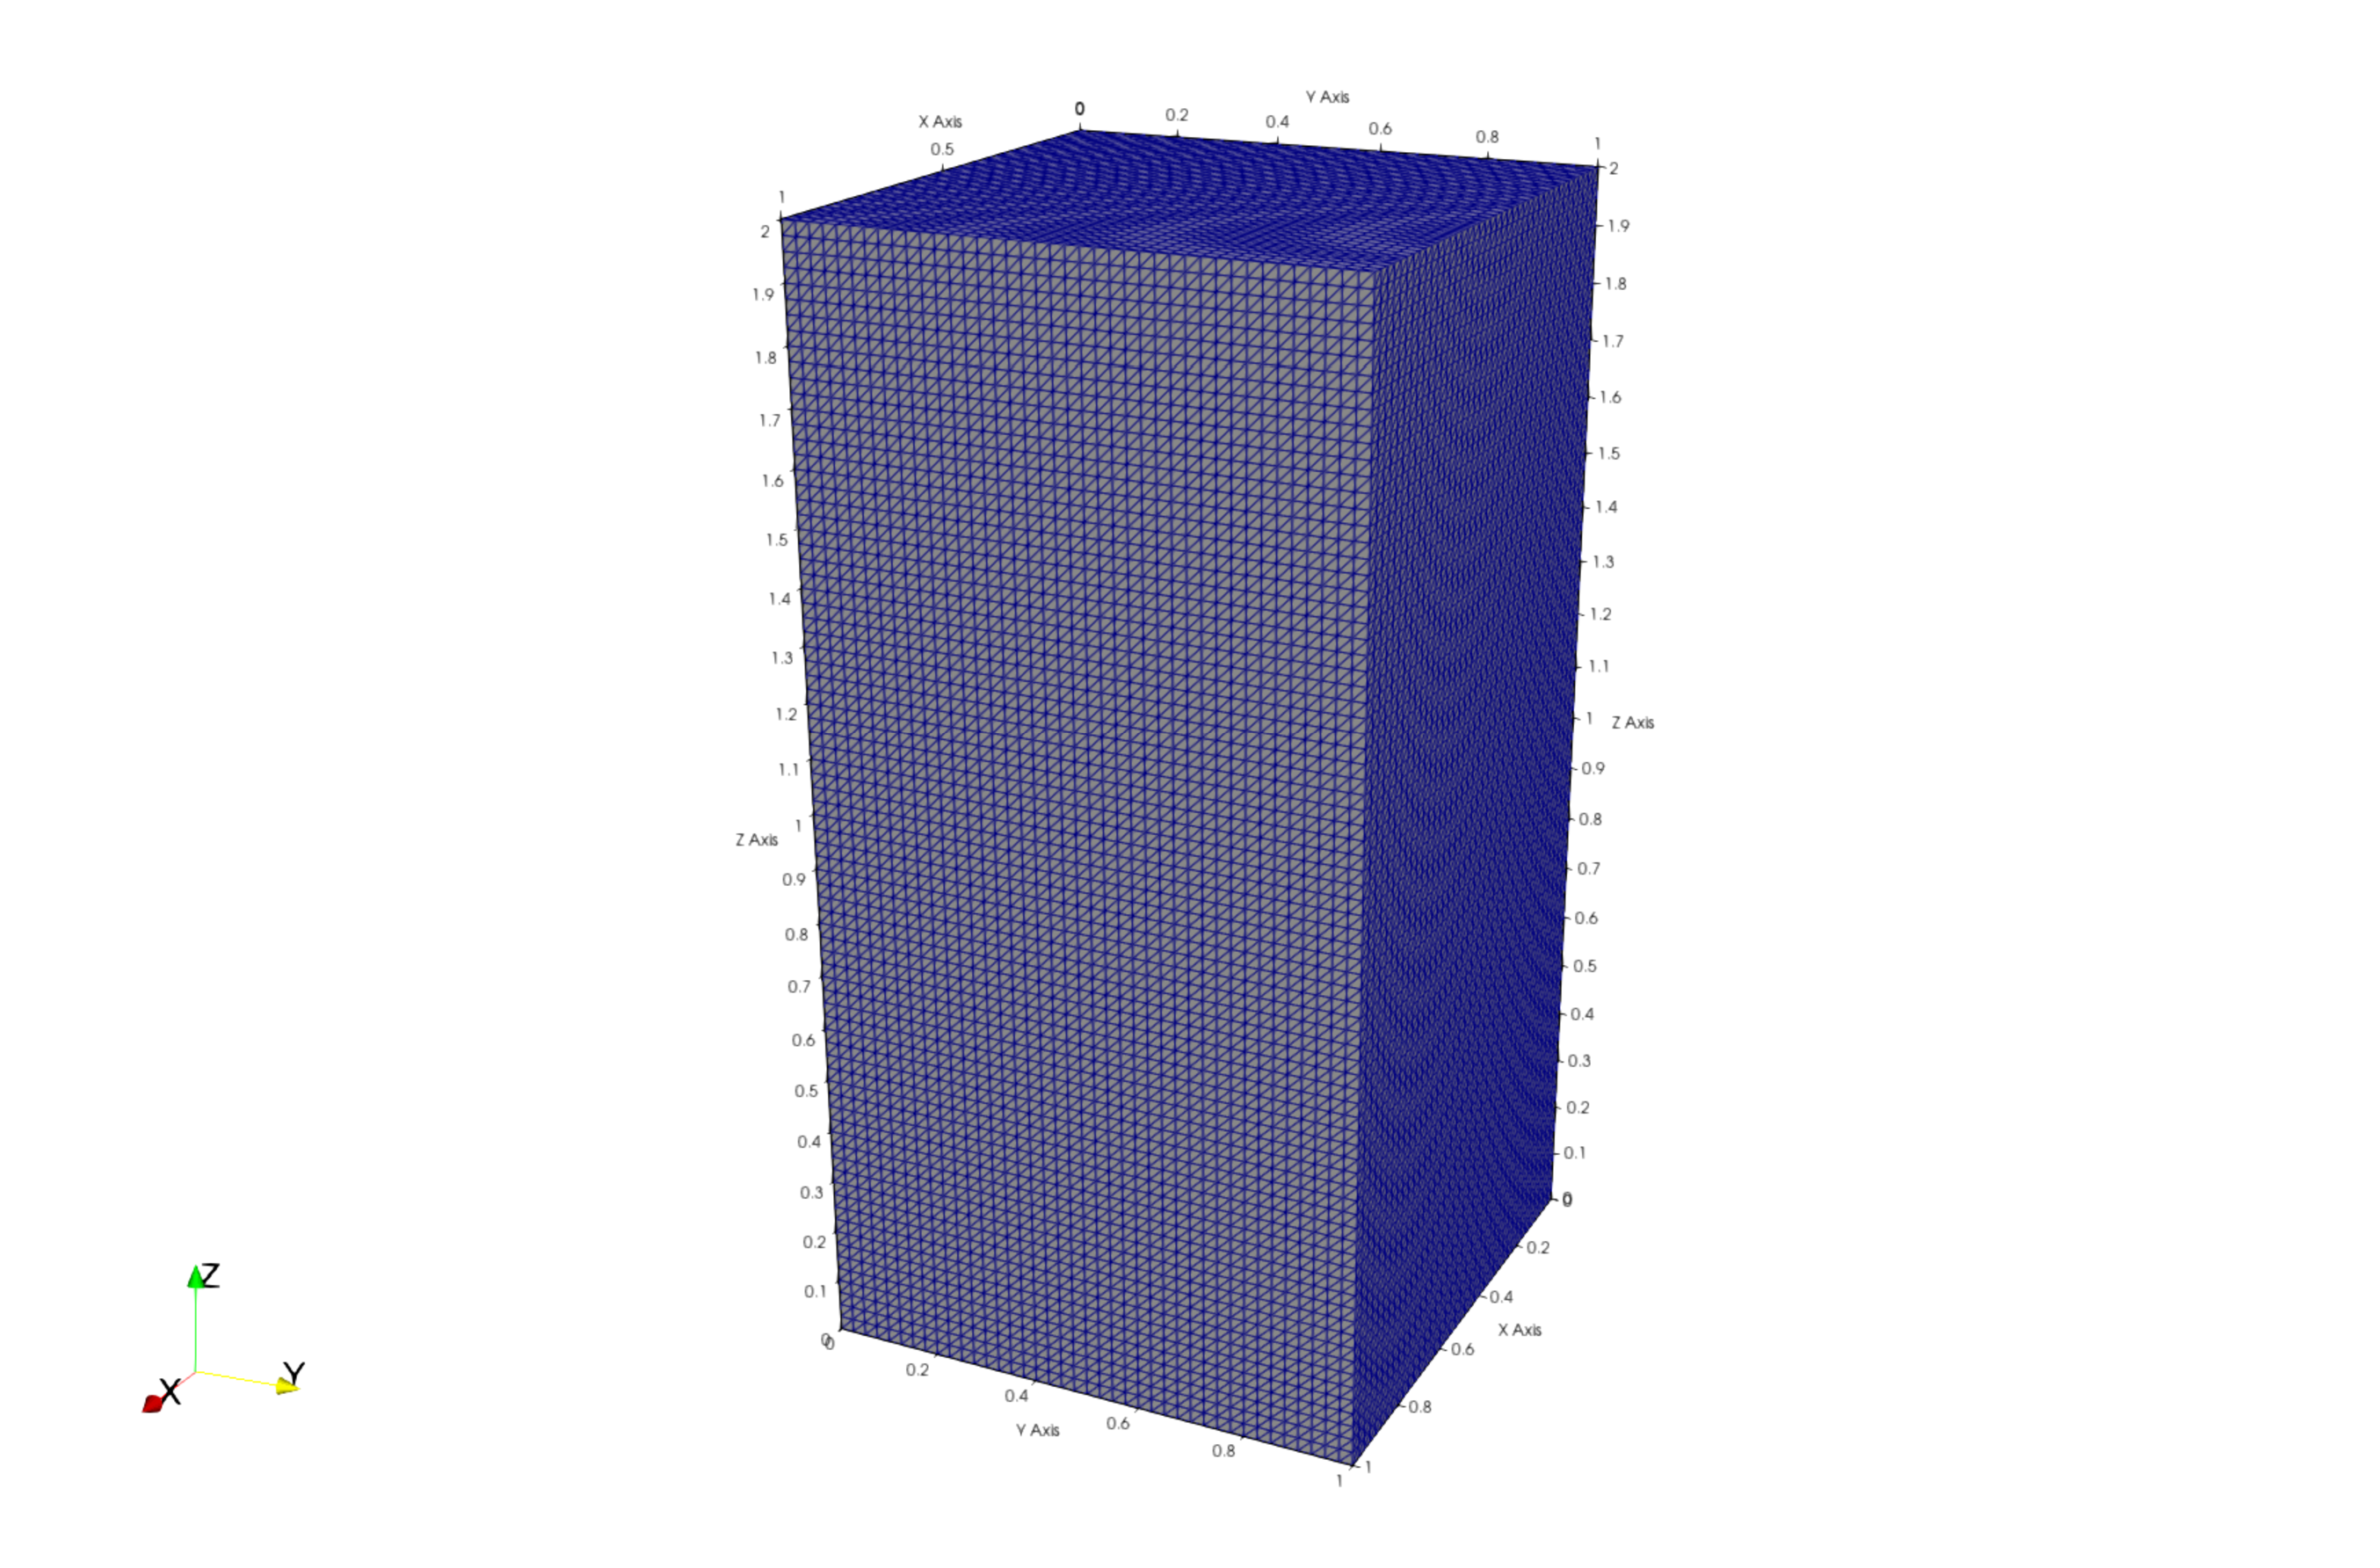
\includegraphics[width=10truecm]{pics/3d-bubble/mesh.pdf}
	\caption{3次元気泡上昇流れの計算メッシュ}
	\label{fig:3d-bubble-mesh}
\end{figure}

Figure \ref{fig:3d-bubble-levelset_t0_3d}に初期状態のレベルセット関数を示す。白い球面が界面である。

\begin{figure}[H]
	\centering
	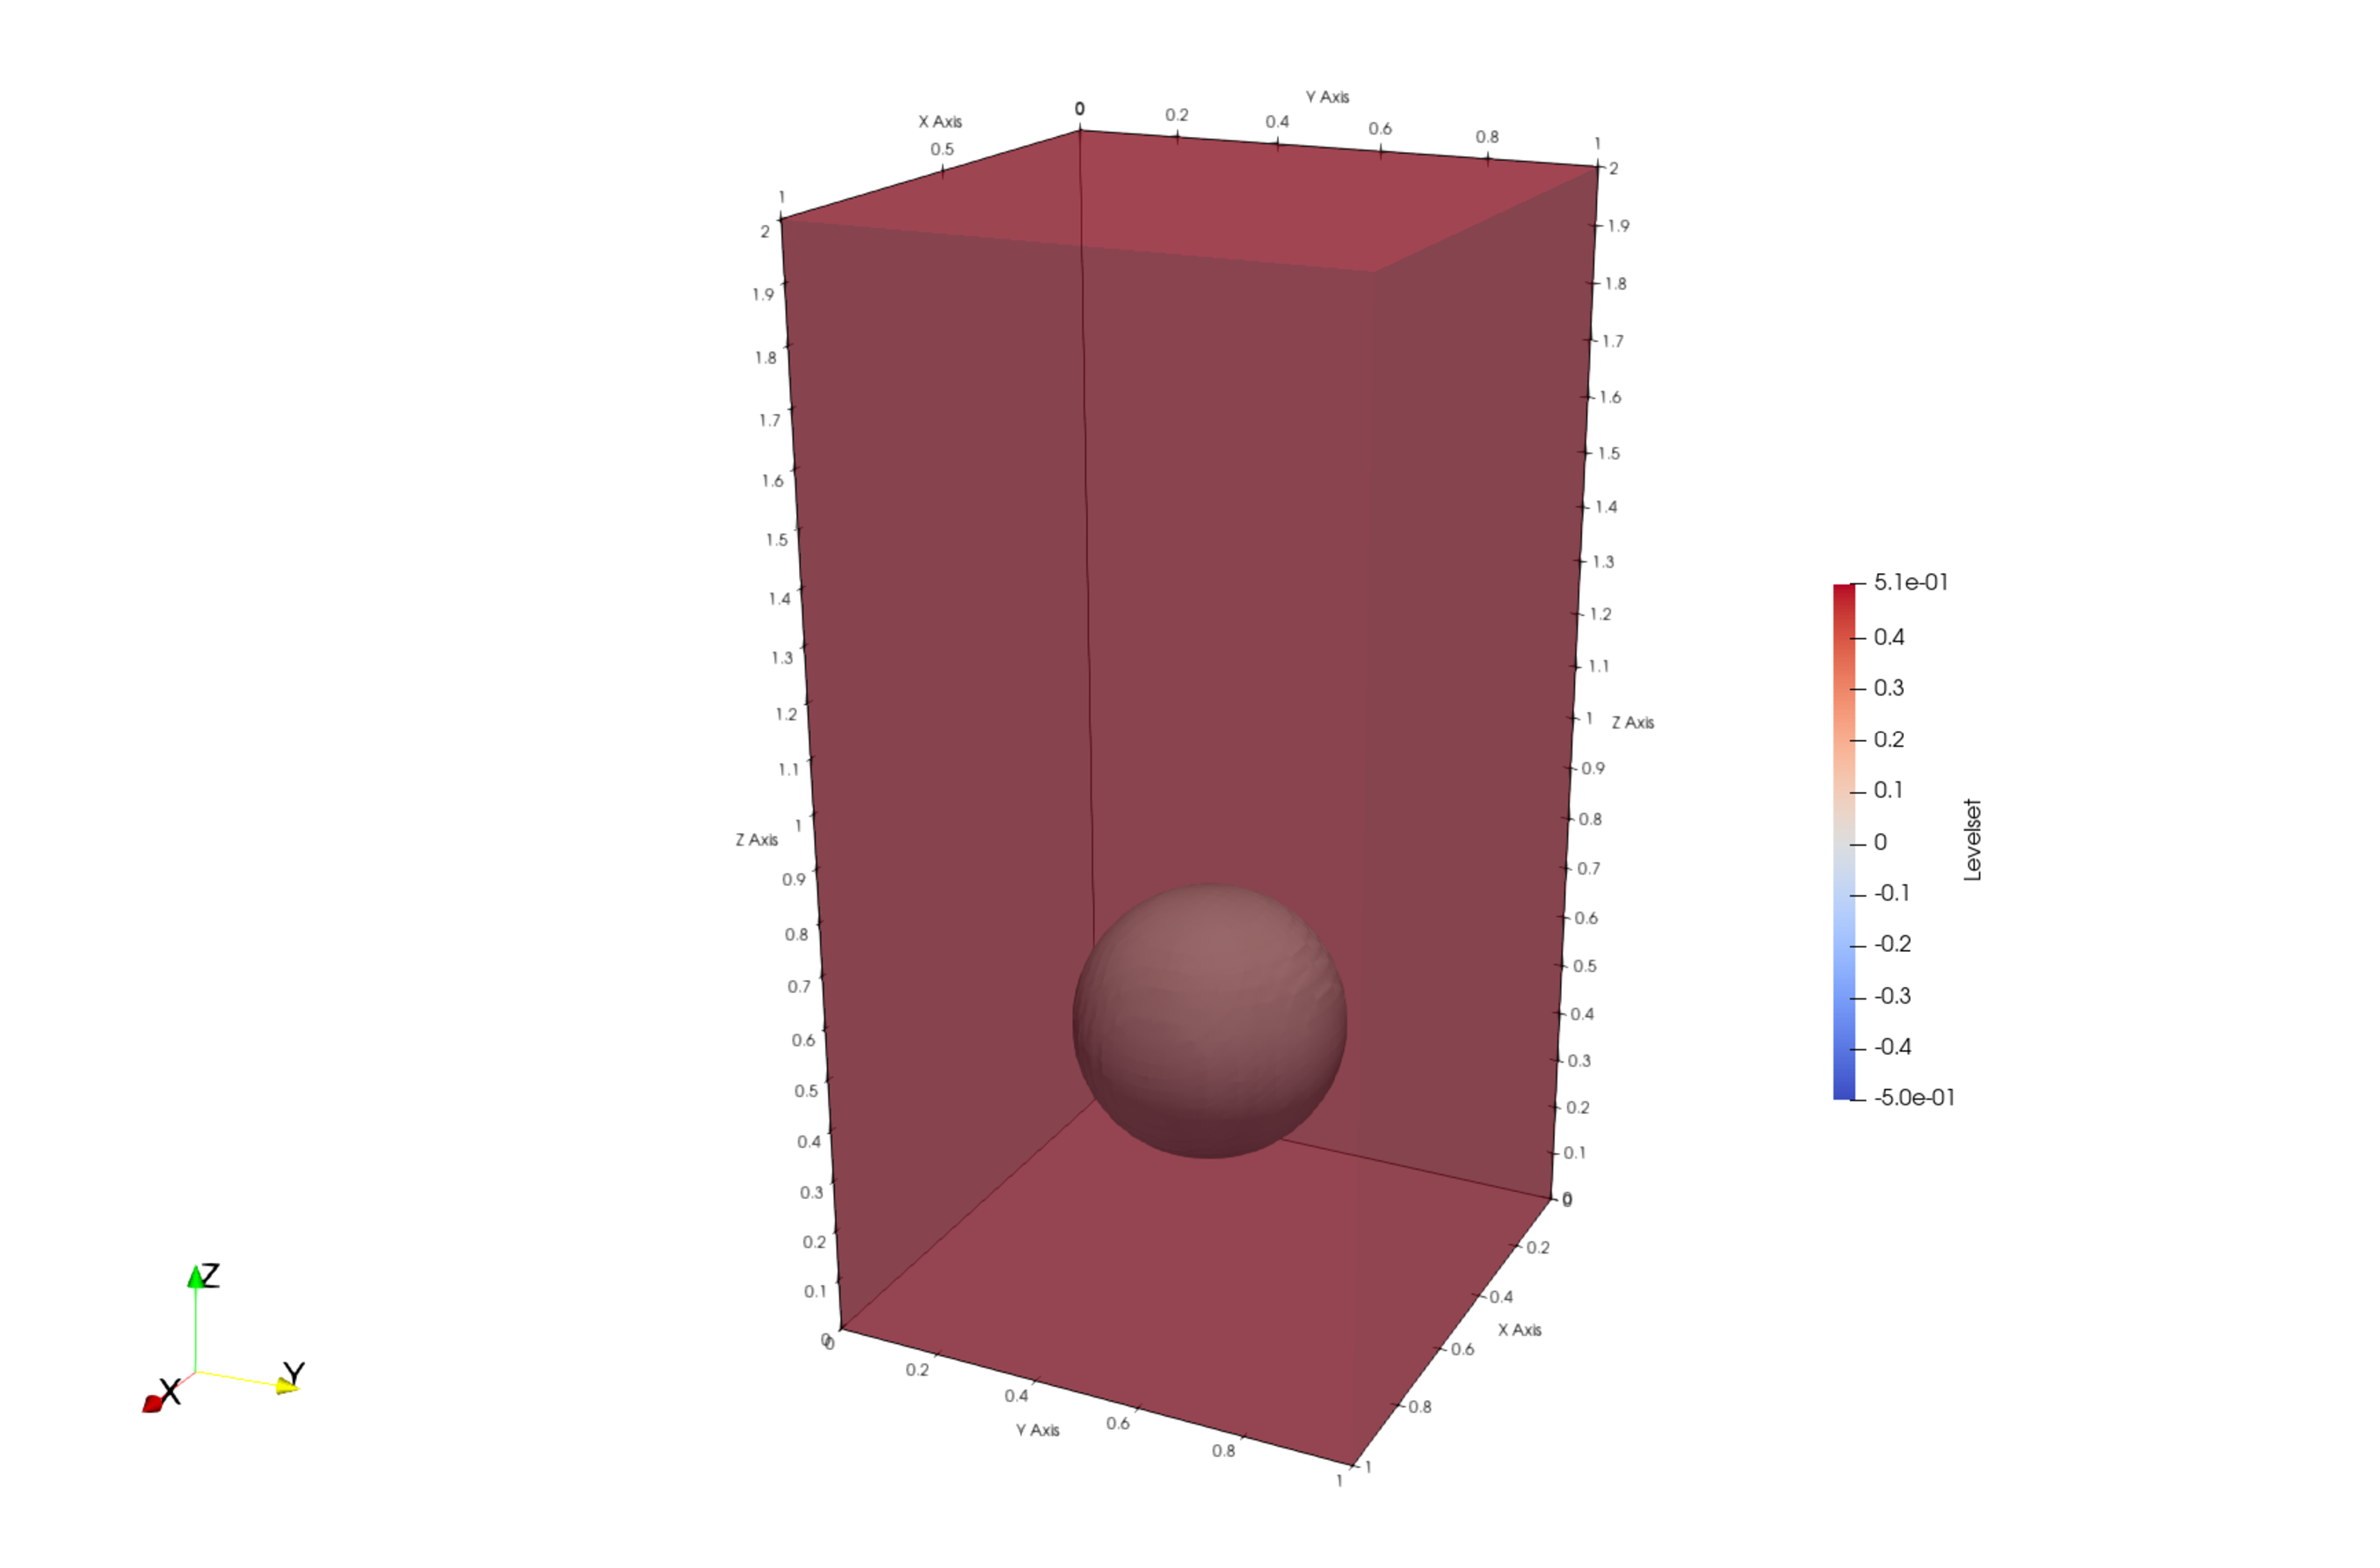
\includegraphics[width=10truecm]{pics/3d-bubble/levelset_t0_3d.pdf}
	\caption{3次元気泡上昇流れの初期状態のレベルセット関数}
	\label{fig:3d-bubble-levelset_t0_3d}
\end{figure}

\subsubsection{解析結果}
気泡上昇流れ問題においては表面張力の影響は大きいと思われるため、表面張力のモデルを導入し計算した結果を示す。

\begin{figure}[H]
	\centering
	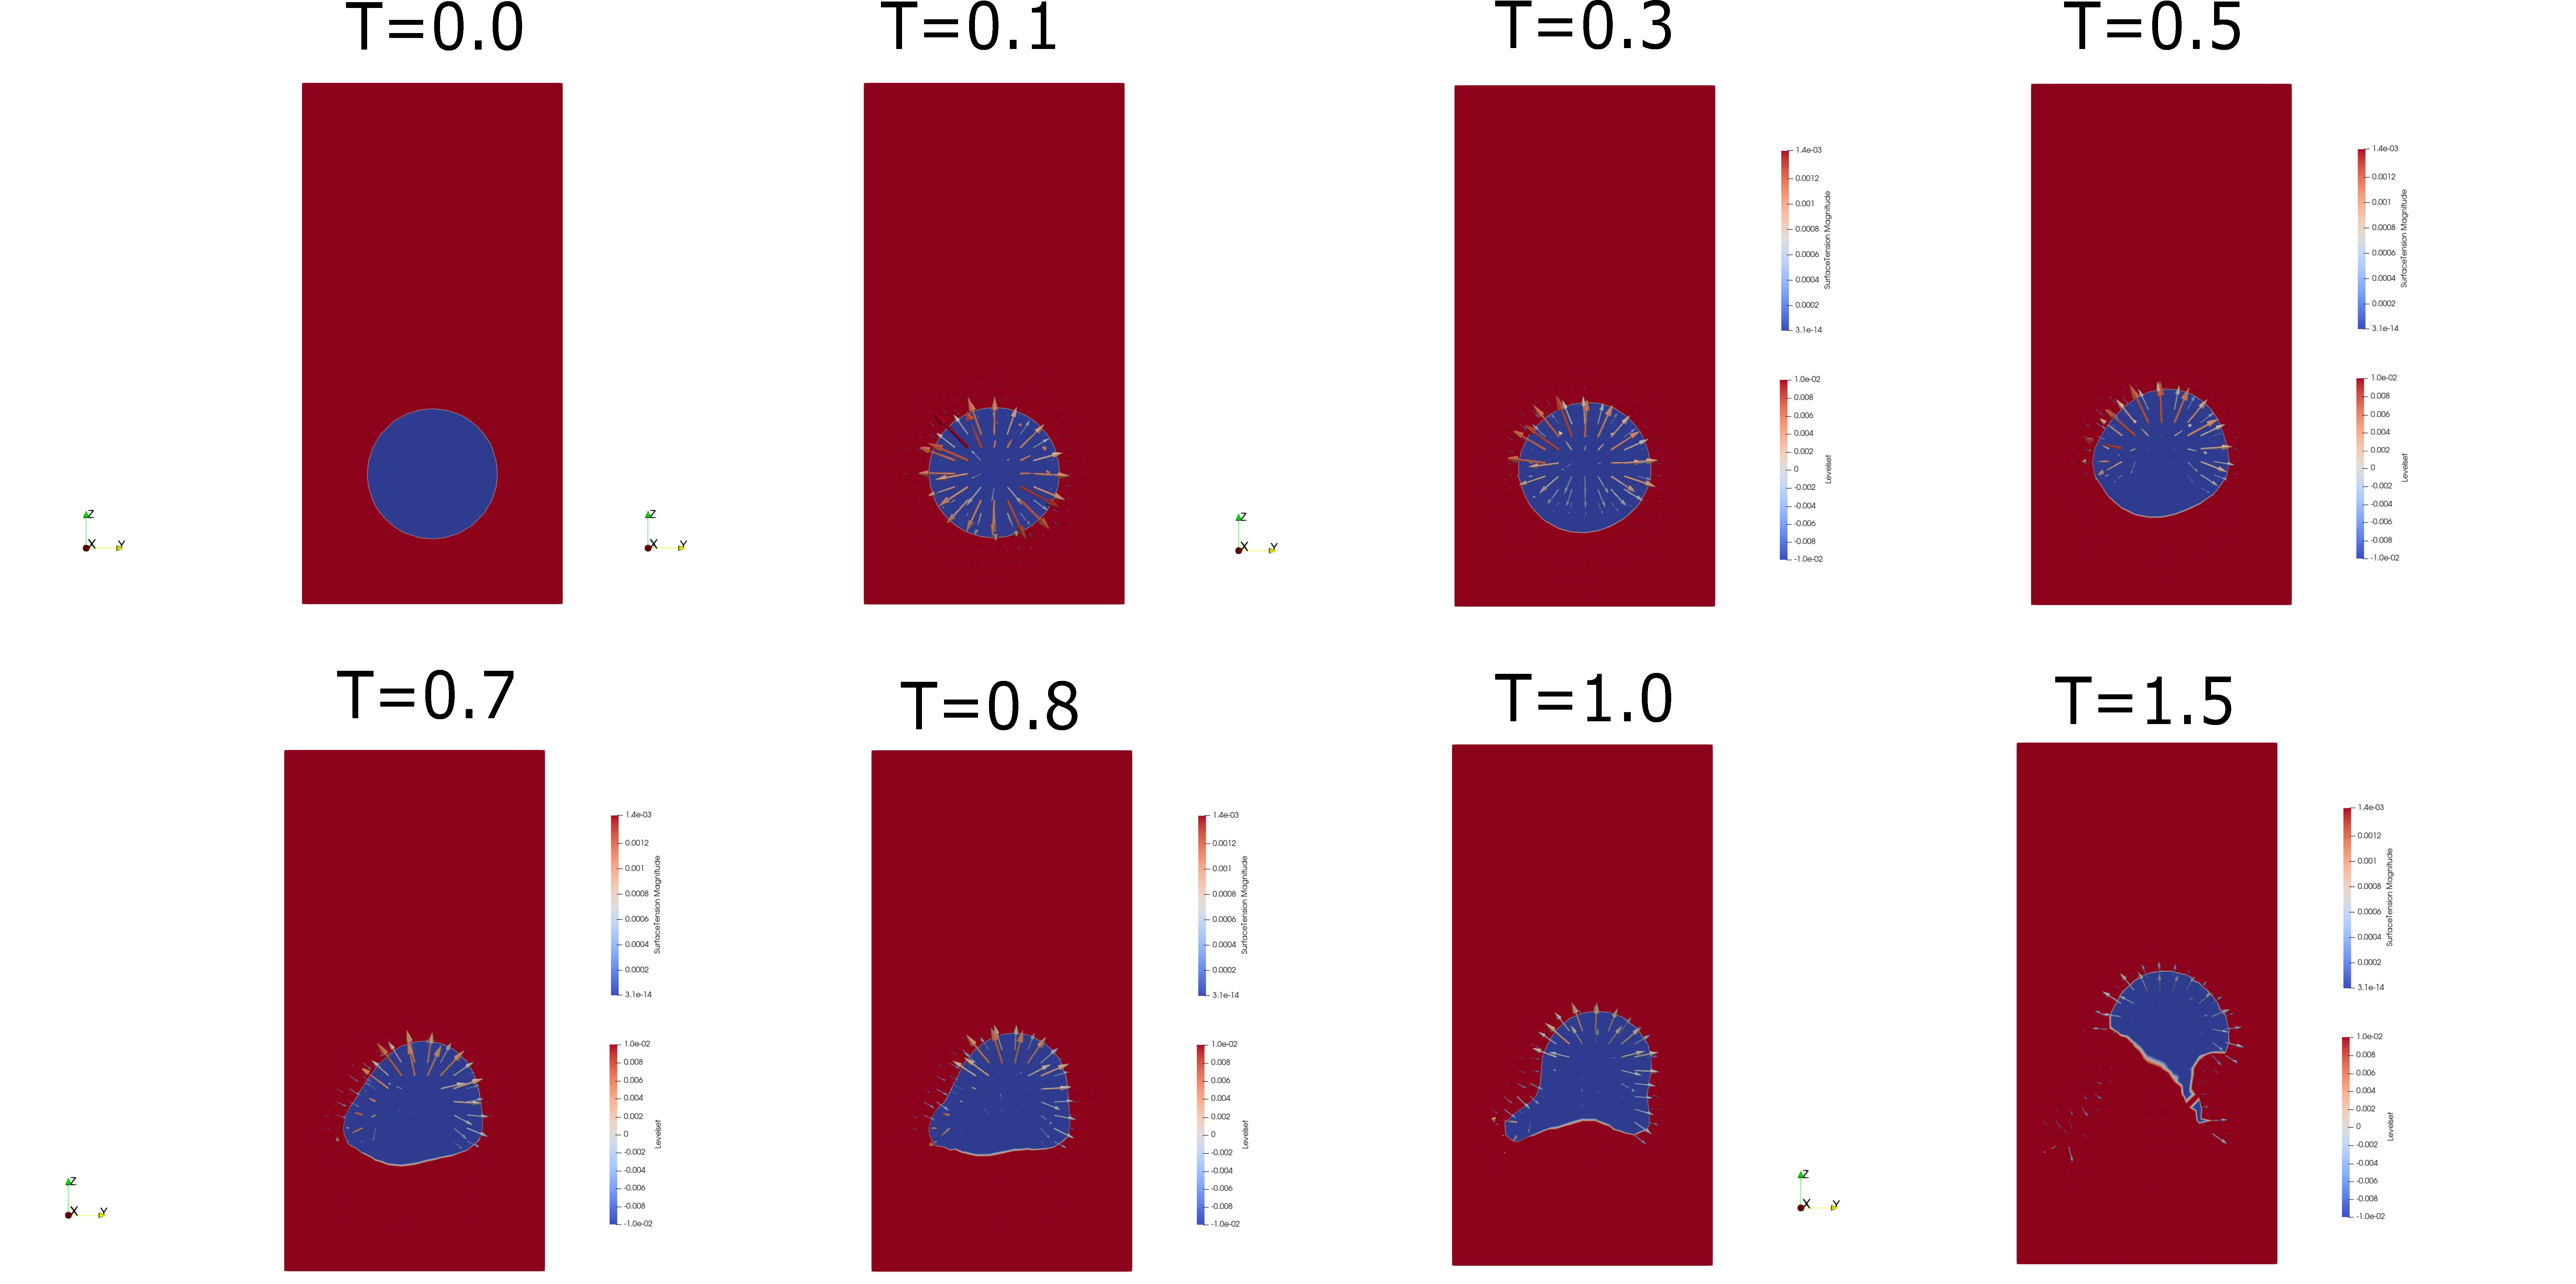
\includegraphics[width=18truecm]{pics/3d-bubble/result_sigma24_5.pdf}
	\caption{3次元気泡上昇流れのレベルセット関数の分布の時間変化($\sigma=24.5$、表面張力あり)}
	\label{fig:3d-bubble_result_sigma24.5}
\end{figure}

\begin{figure}[H]
	\centering
	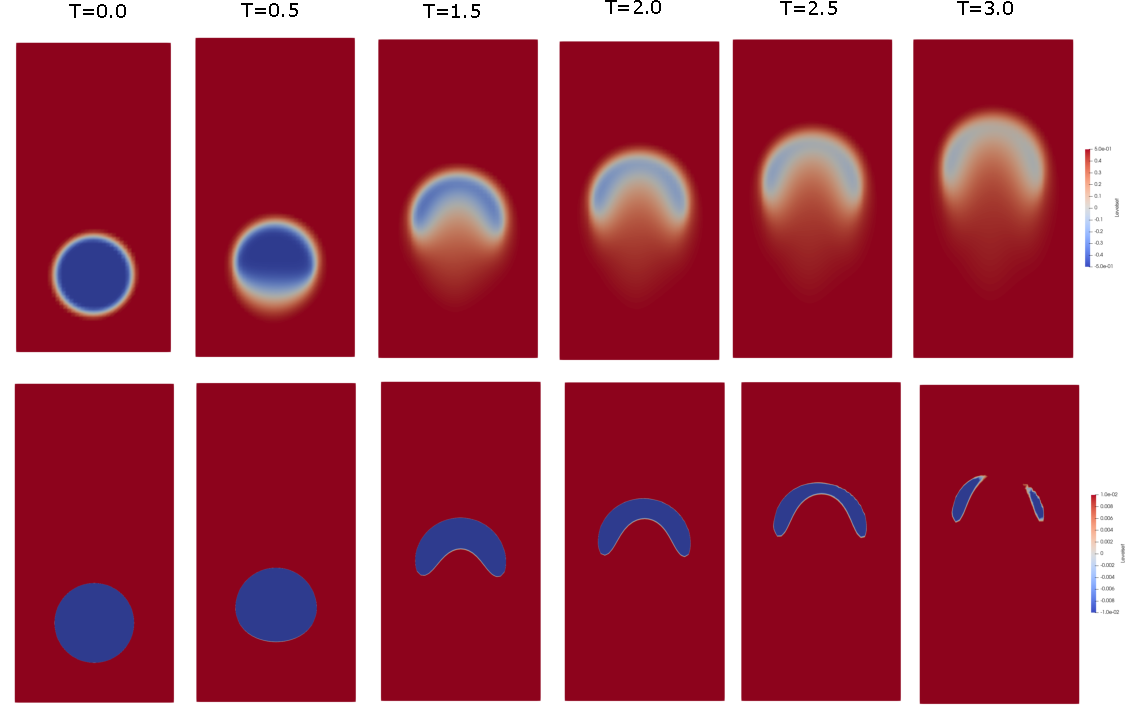
\includegraphics[width=18truecm]{pics/3d-bubble/levelset_t0-3.pdf}
	\caption{3次元気泡上昇流れのレベルセット関数の分布の時間変化($\sigma=0$、表面張力なし)}
	\label{fig:3d-bubble-result_sigma0}
\end{figure}

\begin{figure}[H]
	\centering
	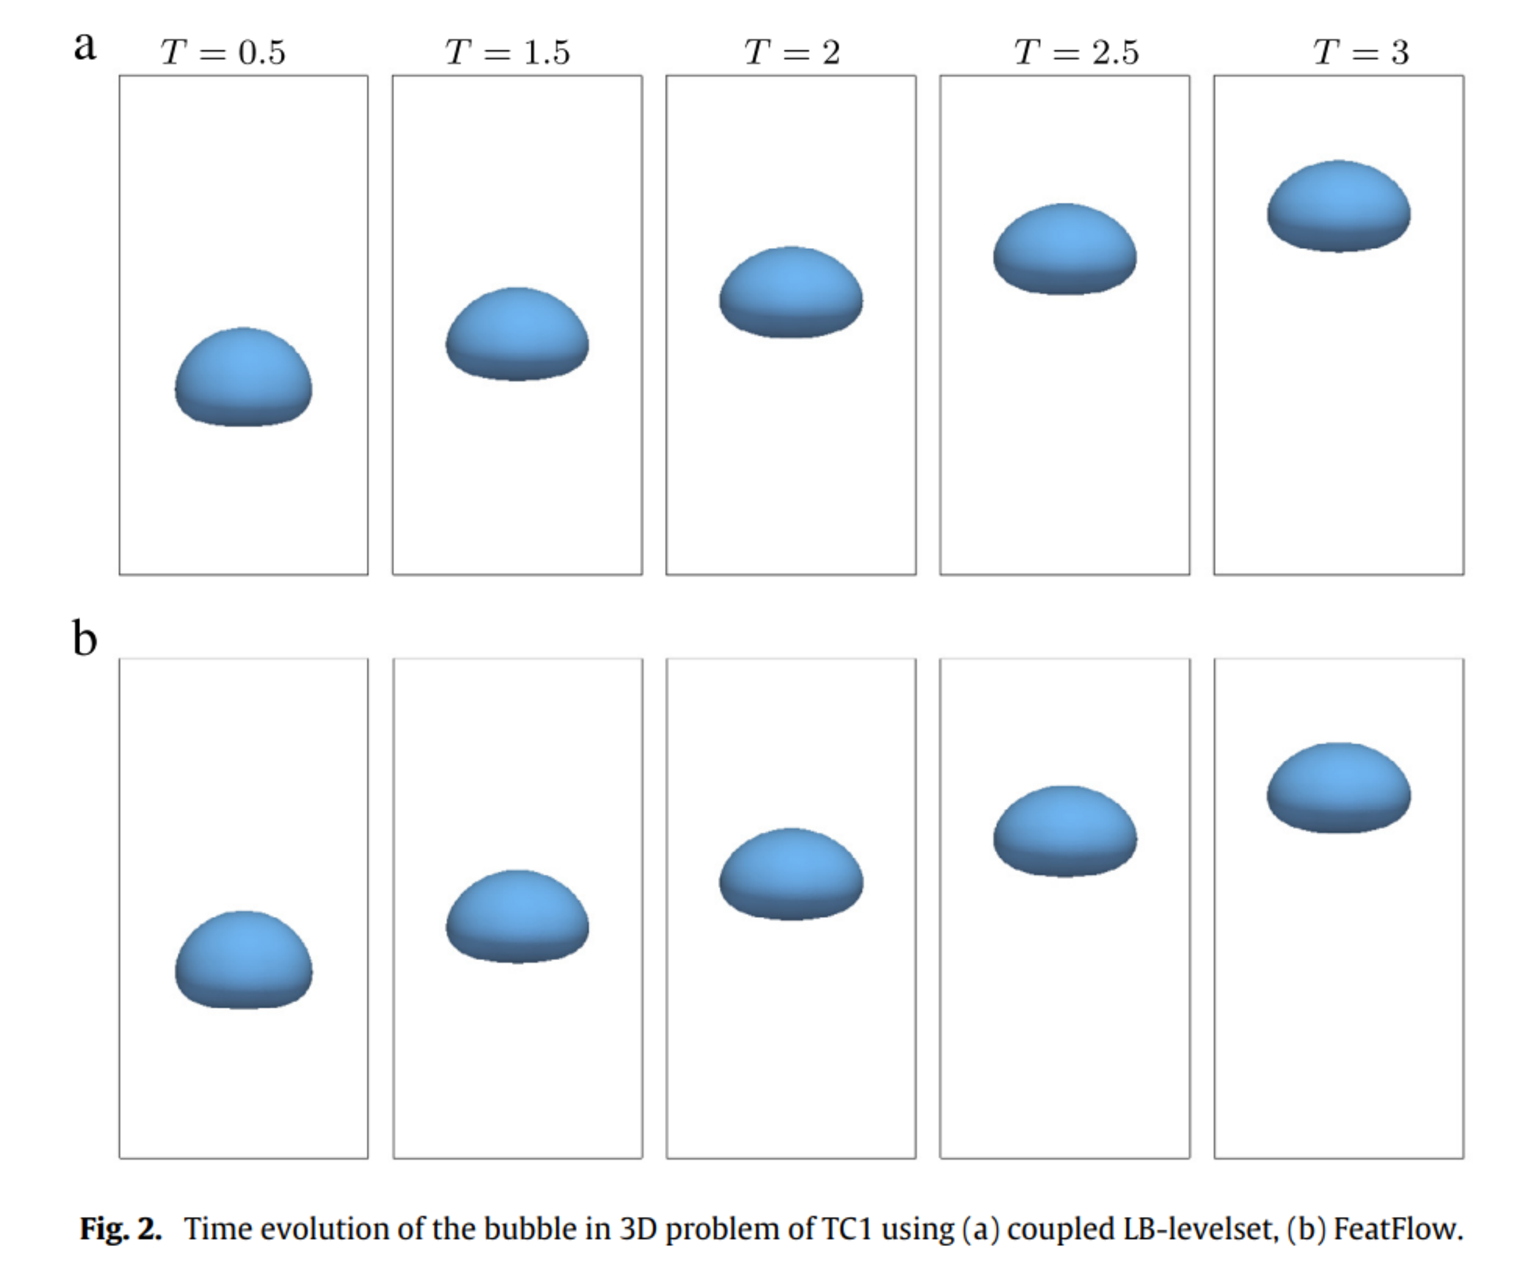
\includegraphics[width=10truecm]{pics/3d-bubble/result-ref.pdf}
	\caption{参考文献結果($\sigma=24.5$)\cite{Safi2017}}
	\label{fig:3d-bubble-result-ref}
\end{figure}